\section{Architettura del sistema}
SWIMv2 è sviluppato secondo l'architettura client-server, e quest'ultimo secondo il pattern MVC, in modo da tenere nettamente separati lo stato del sistema, la logica di
business e l'interfaccia grafica. In particolare, per quanto riguarda il client, possiamo immaginare che esso sia un comunissimo browser che manda delle richieste ad un server ed
elabora le sue risposte, mostrando all'utente le informazioni desiderate tramite la view che gli viene passata. Il server invece è locale (fondamentalmente http://127.0.0.1:8080),
ospita il database e la logica di business e fornisce un'interfaccia grafica personalizzata a seconda dello stato del sistema; tale stato varia a seconda dei comandi ricevuti dal
client, ma non in modo arbitrario: il controller si occupa di mantenere il DB in uno stato consistente e di comporre volta per volta l'HTML da passare al browser; a questo proposito,
particolare importanza hanno le servlet, componenti che appunto generano le pagine web dinamiche che l'utente vede. Il server, come già specificato è JBoss AS 5, un'implementazione
open source della piattaforma J2EE.
\\
La seguente figura rappresenta graficamente l'architettura del sistema:
\vspace{0.5cm}
\center
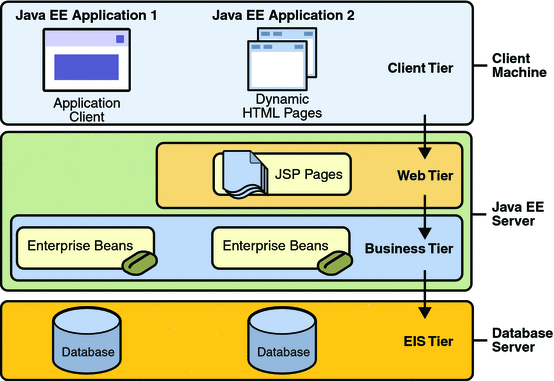
\includegraphics[scale=2.5]{J2EE.png}
\pagebreak